\documentclass[problem]{mcs}

\begin{pcomments}
  \pcomment{PS_3color_crossover_SAT}
  \pcomment{by ARM 4/6/14}
  \pcomment{TBA: revise to use simpler 3color-paterson-crossover with
    solns 3color-paterson-same-color 3color-paterson-diff-color}
\end{pcomments}

\pkeywords{
  coloring
  planar
  3-coloring
}

%%%%%%%%%%%%%%%%%%%%%%%%%%%%%%%%%%%%%%%%%%%%%%%%%%%%%%%%%%%%%%%%%%%%%
% Problem starts here
%%%%%%%%%%%%%%%%%%%%%%%%%%%%%%%%%%%%%%%%%%%%%%%%%%%%%%%%%%%%%%%%%%%%%

\begin{problem}
The 3-coloring problem for planar graphs turns out to be no easier
than the 3-coloring problem for arbitrary graphs.  This claim follows
very simply from the existence of a ``3-color cross-over gadget.''
Such a gadget is a planar graph whose outer face is a cycle with four
designated vertices $u,v,w,x$ occurring in clockwise order such that

\begin{enumerate}[(i)]

\item\label{exist3coloring} Any assignment of colors to vertices $u$ and $v$ can be
  completed into a 3-coloring of the gadget.
\item\label{colors-cross} In every 3-coloring of the gadget, the colors of $u$ and $w$ are
  the same, and the colors of $v$ and $x$ are the also same.

\end{enumerate}

Figure~\ref{fig:3color-gadget} shows such a 3-color cross-over
gadget.\footnote{The original such gadget and reduction of 3-colorability to planar
  3-colorability were due to Larry Stockmeyer~\cite{Stockmeyer73}.  The current simplified gadget is due to M.S. Paterson.}

\begin{figure}%\inbook{[h]}
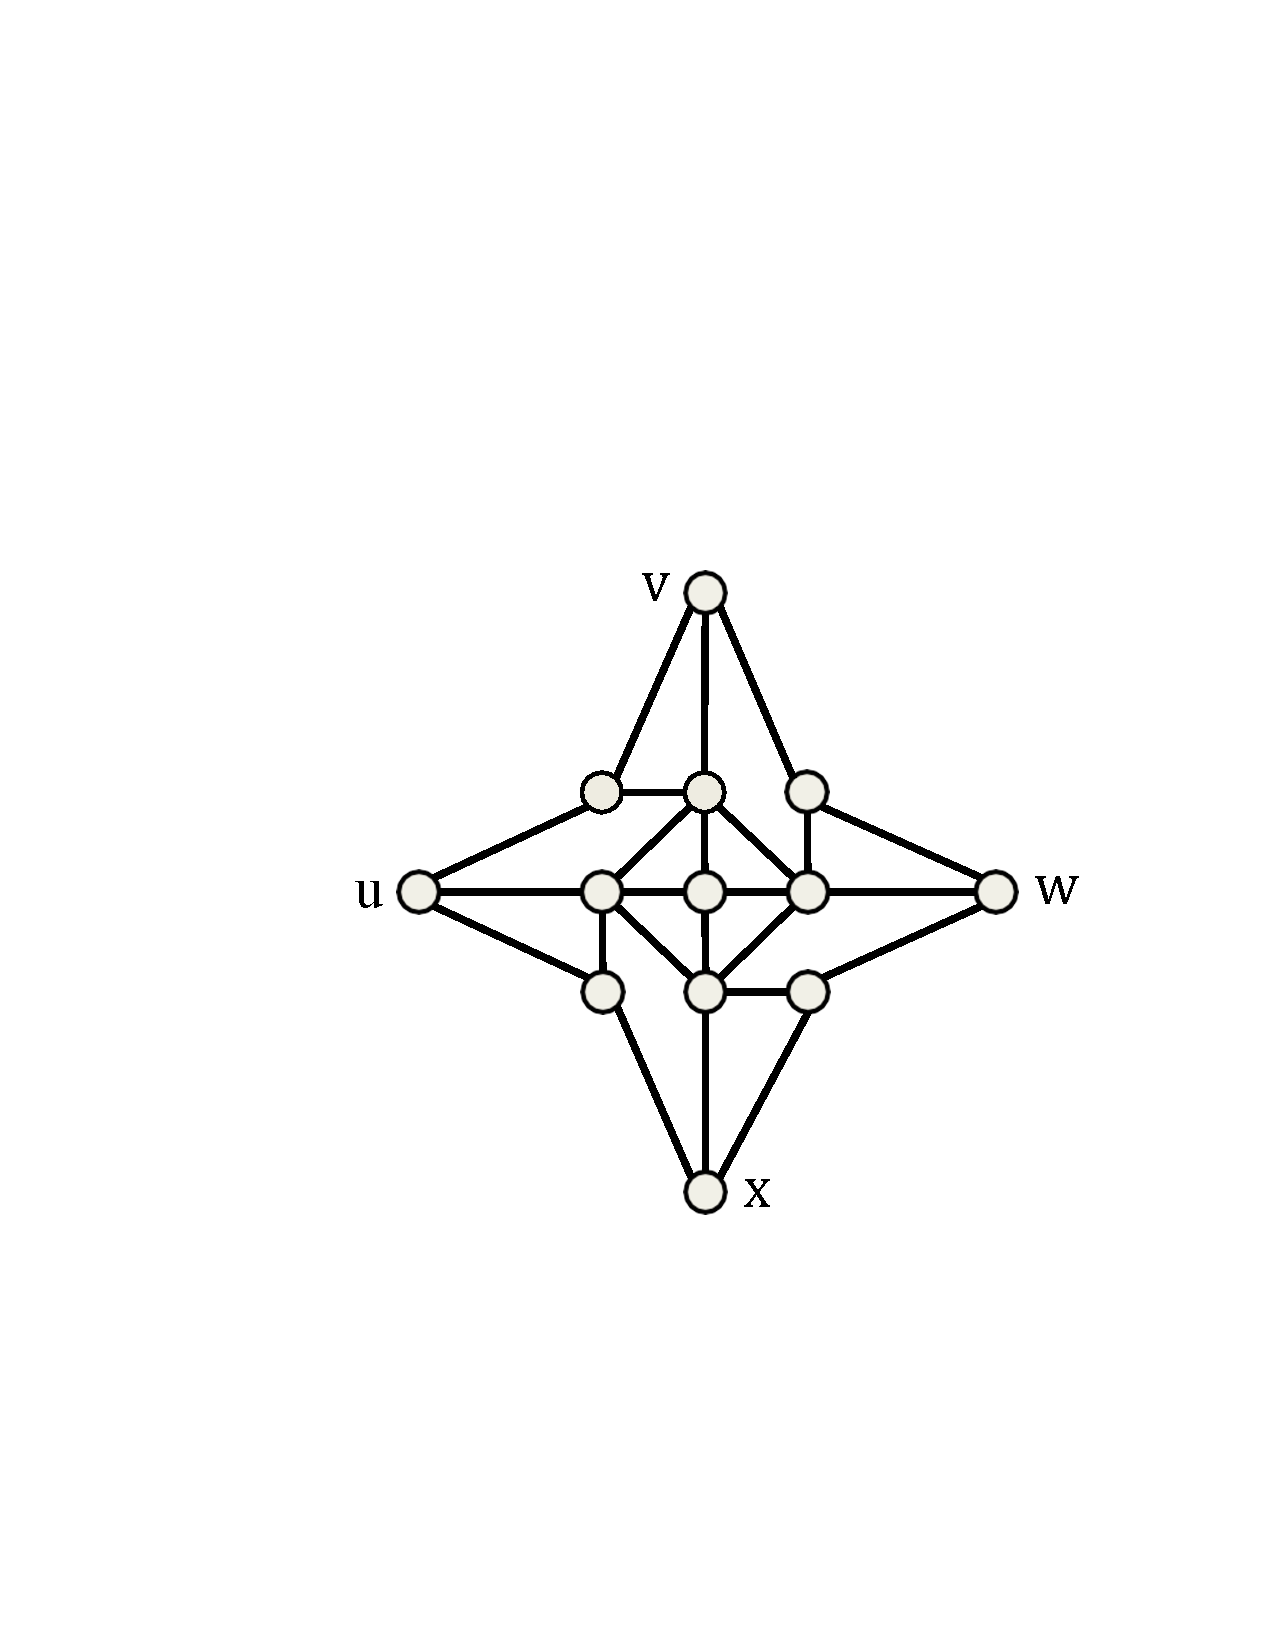
\includegraphics[width=2.5in]{3color-paterson-crossover}
\caption{A 3-color cross-over gadget.}
\label{fig:3color-gadget}
\end{figure}

So to find a 3-coloring for \emph{any} simple graph, simply draw it in
the plane with edges crossing as needed, and then replace each
occurrence of an edge crossing by a copy of the gadget as shown in
Figure~\ref{fig:replace-crossing}.  This yields a planar graph which
has a 3-coloring iff the original graph had one.

\begin{figure}%\inbook{[h]}
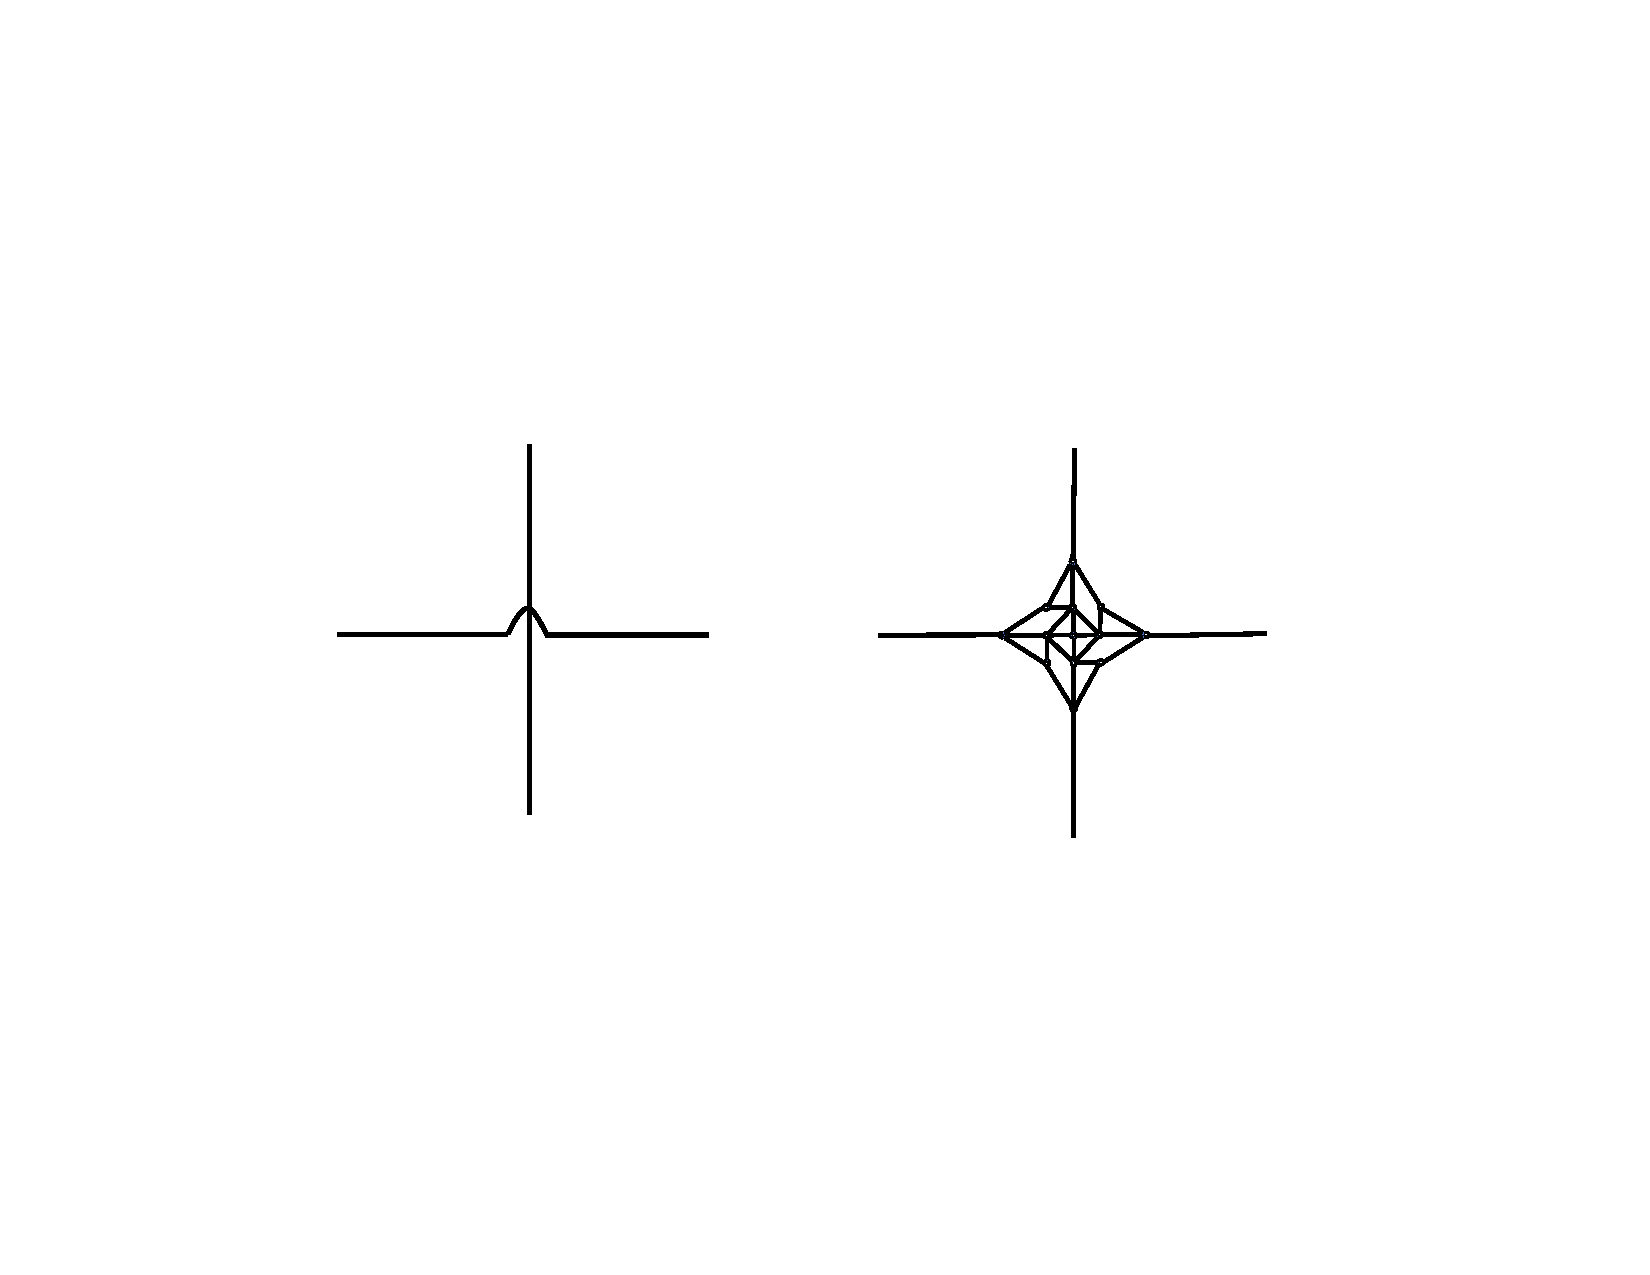
\includegraphics[width=4.0in]{3color-crossing}
%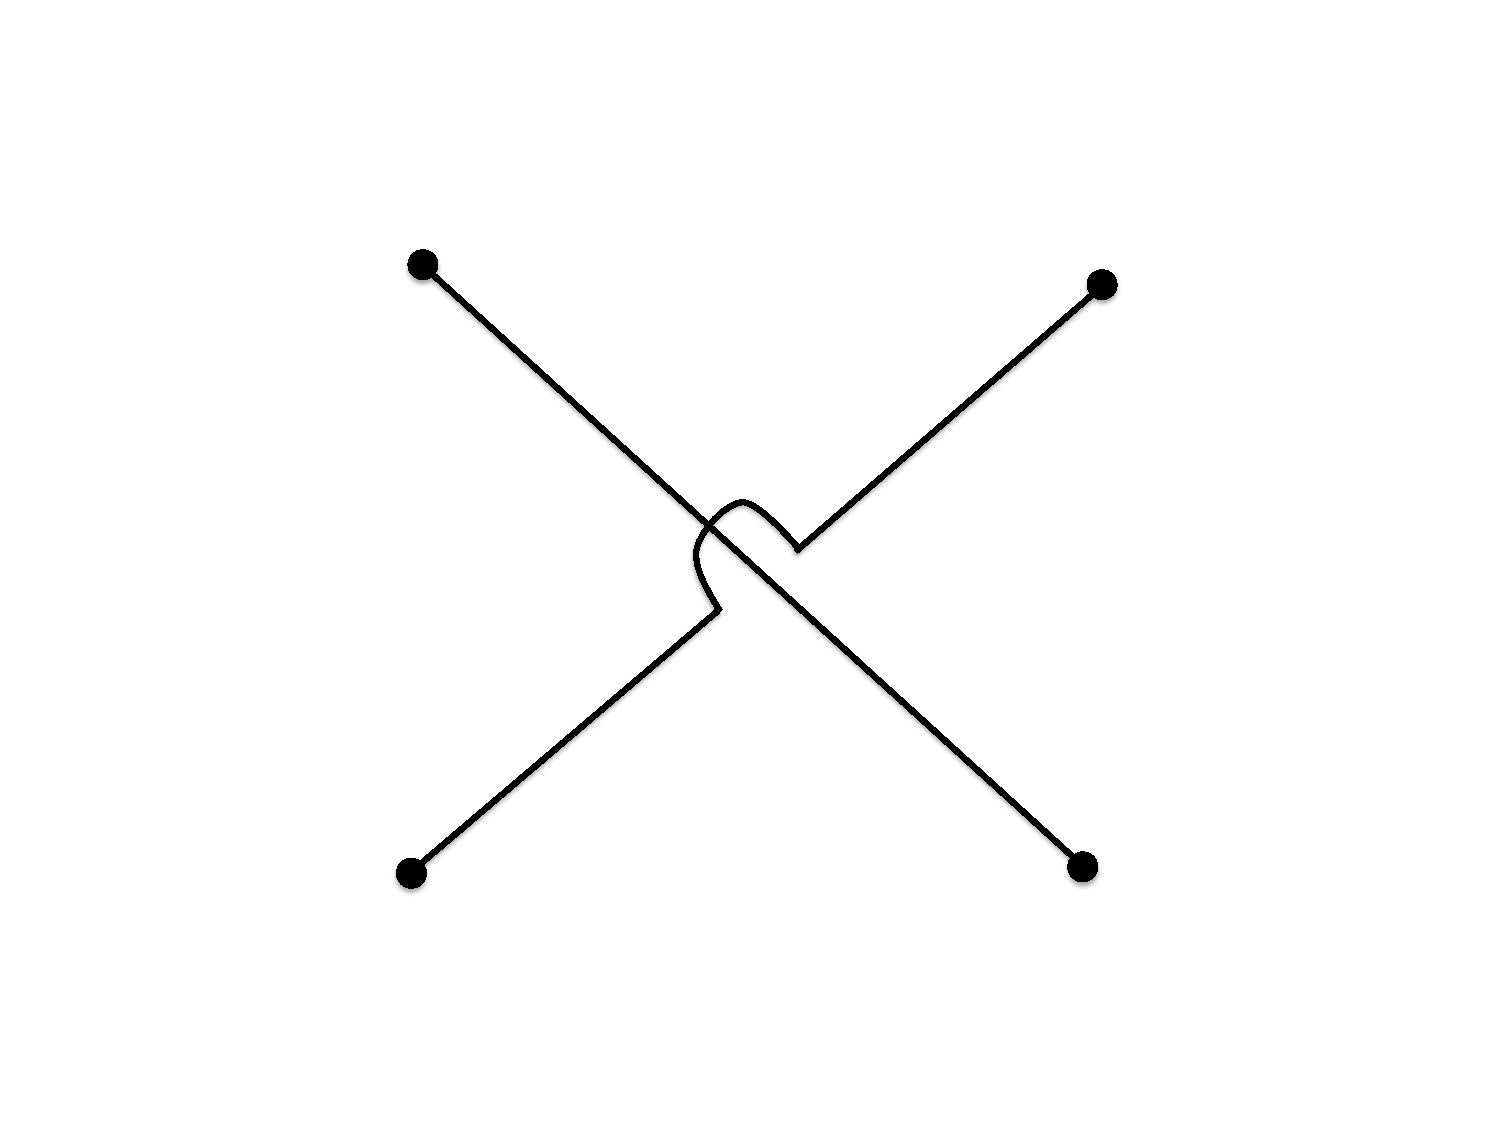
\includegraphics[width=2.3in]{edge-crossing} 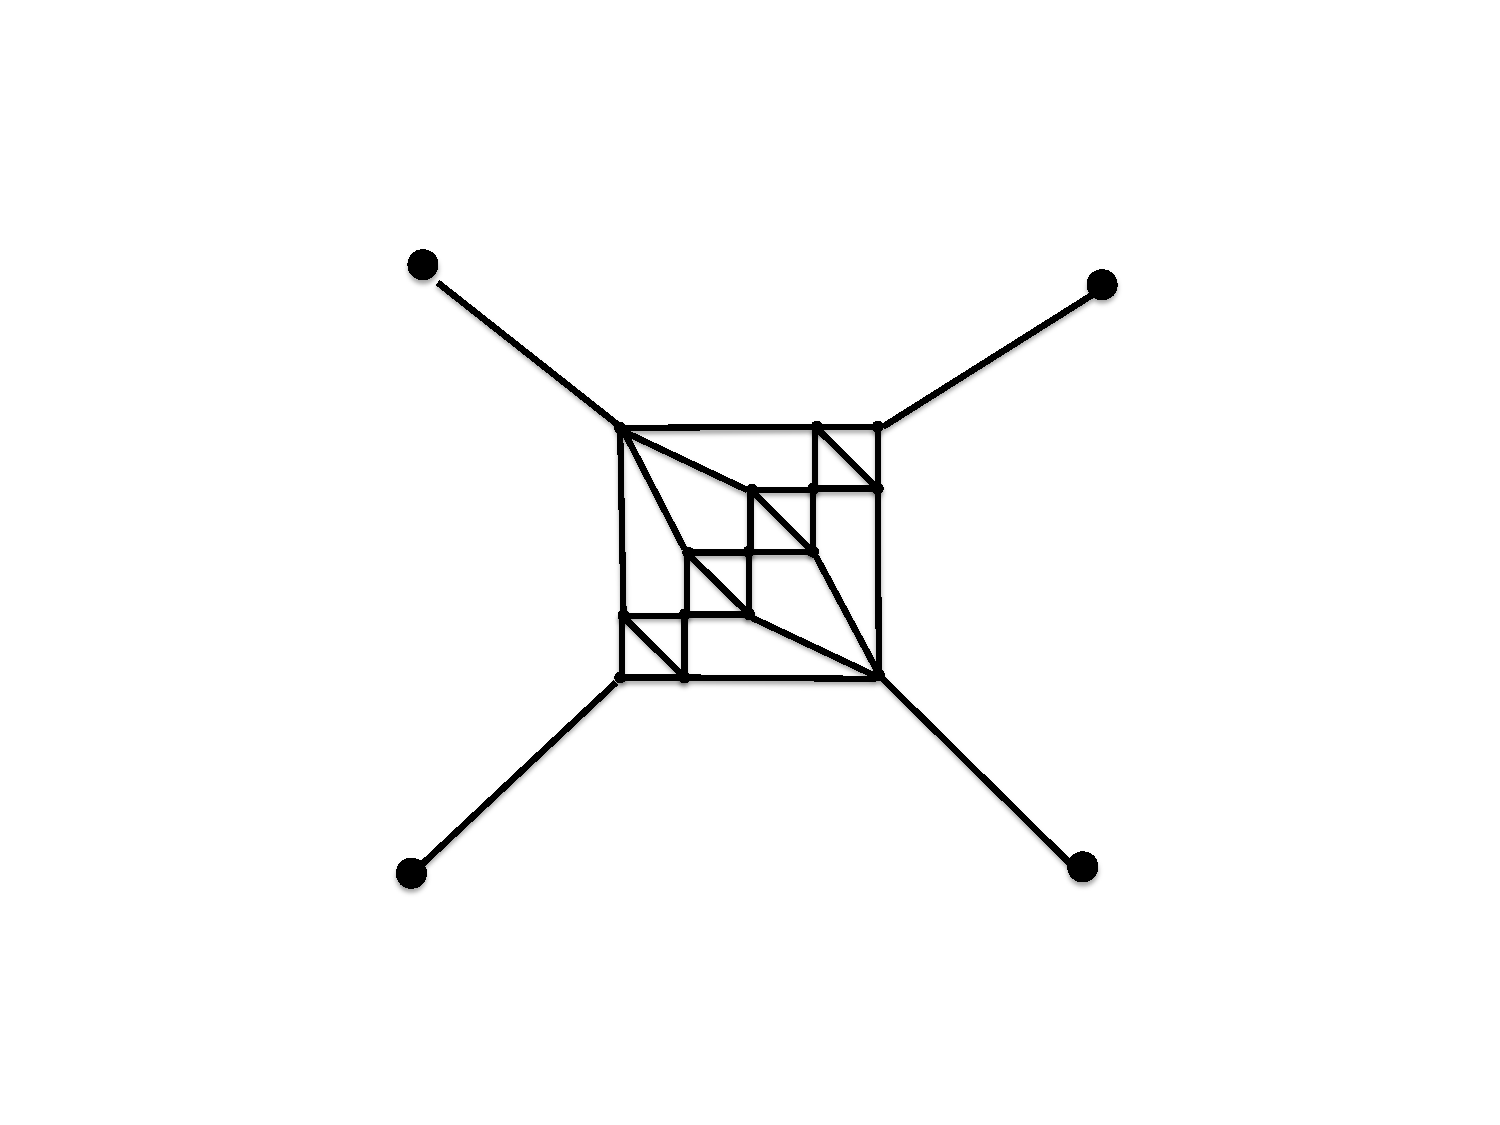
\includegraphics[width=2.3in]{3color-gadget-crossing}
\caption{Replacing an edge-crossing with a planar gadget.}
\label{fig:replace-crossing}
\end{figure}

\bparts

\ppart\label{verify3coloring} Prove that the graph in
Figure~\ref{fig:3color-gadget} satisfies
condition~\eqref{exist3coloring} by exhibiting the claimed
3-colorings.

\instatements{
\hint Only two colorings are needed, one where $u$ and $v$ are the
same color and another where they are not the same color.
}

\begin{solution}
\begin{figure}%\inbook{[h]}
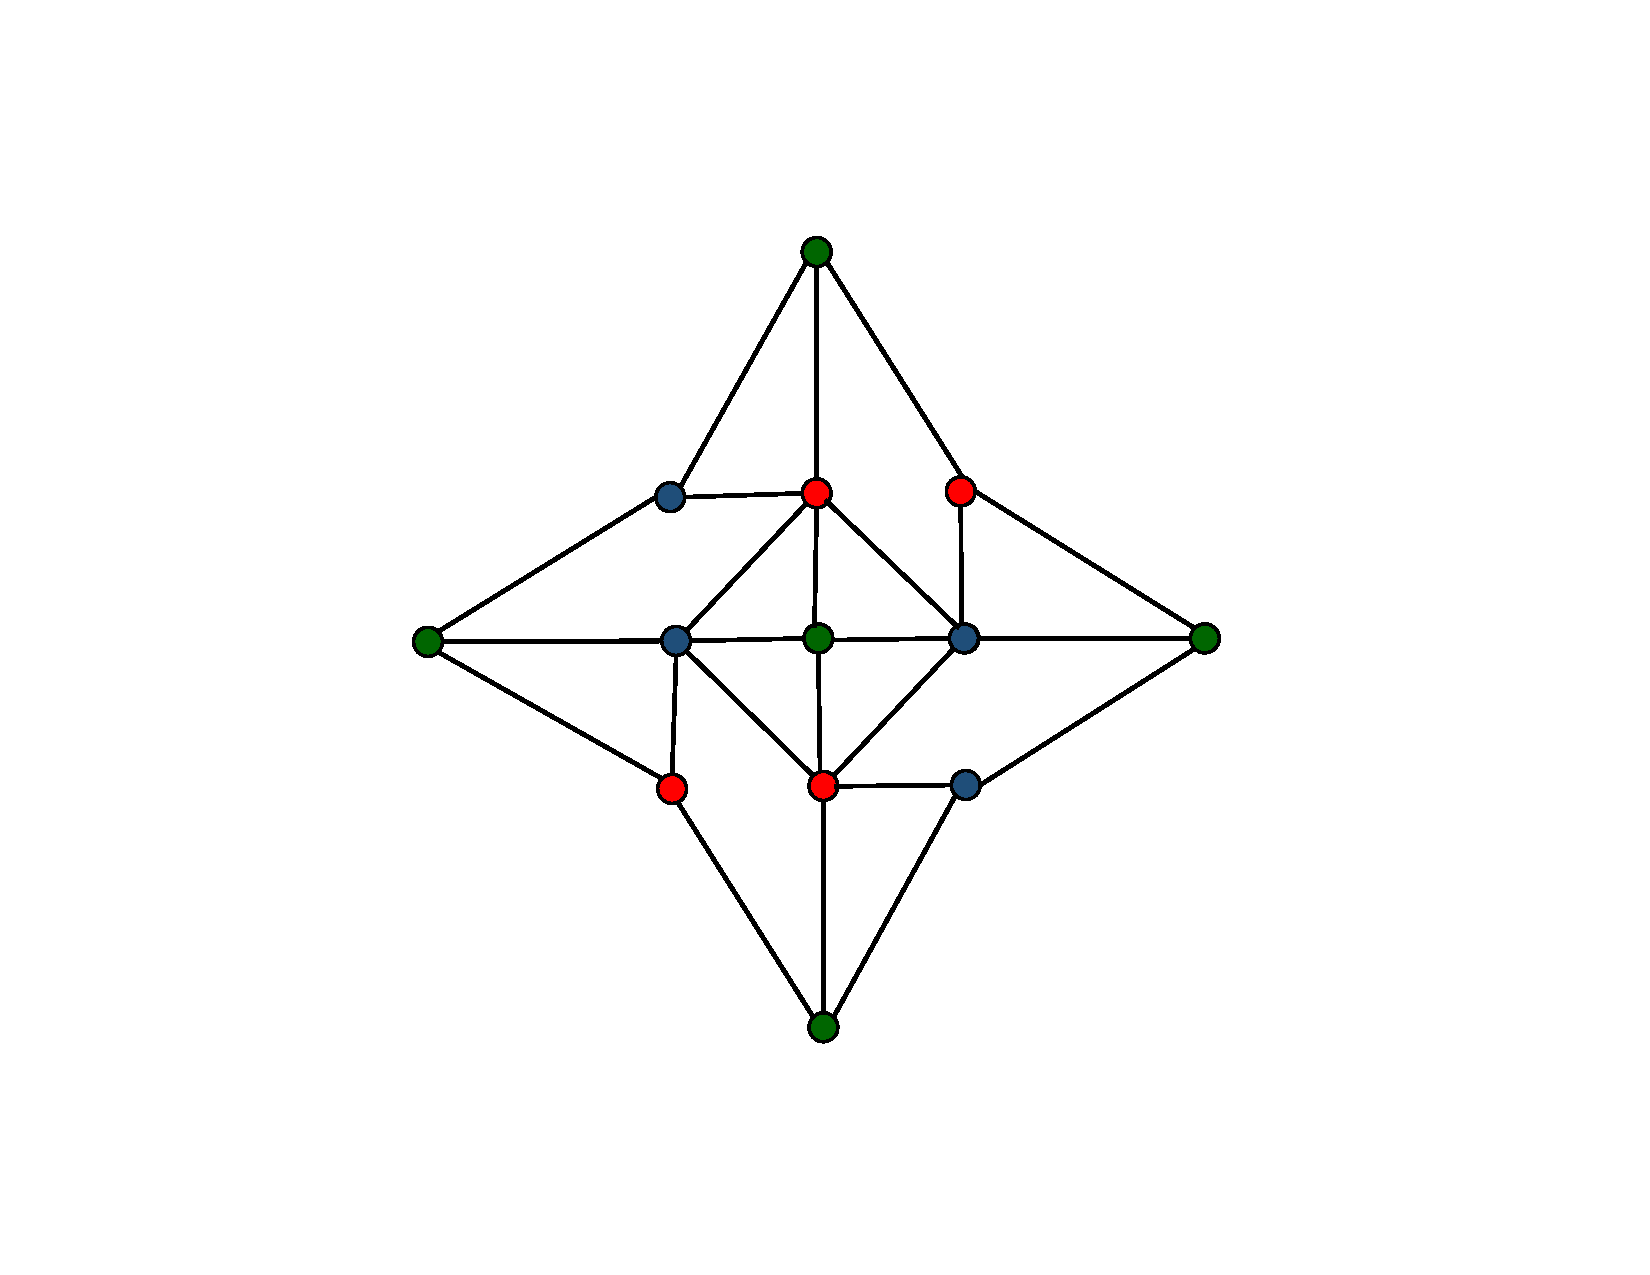
\includegraphics[width=4.0in]{3color-paterson-same-color} 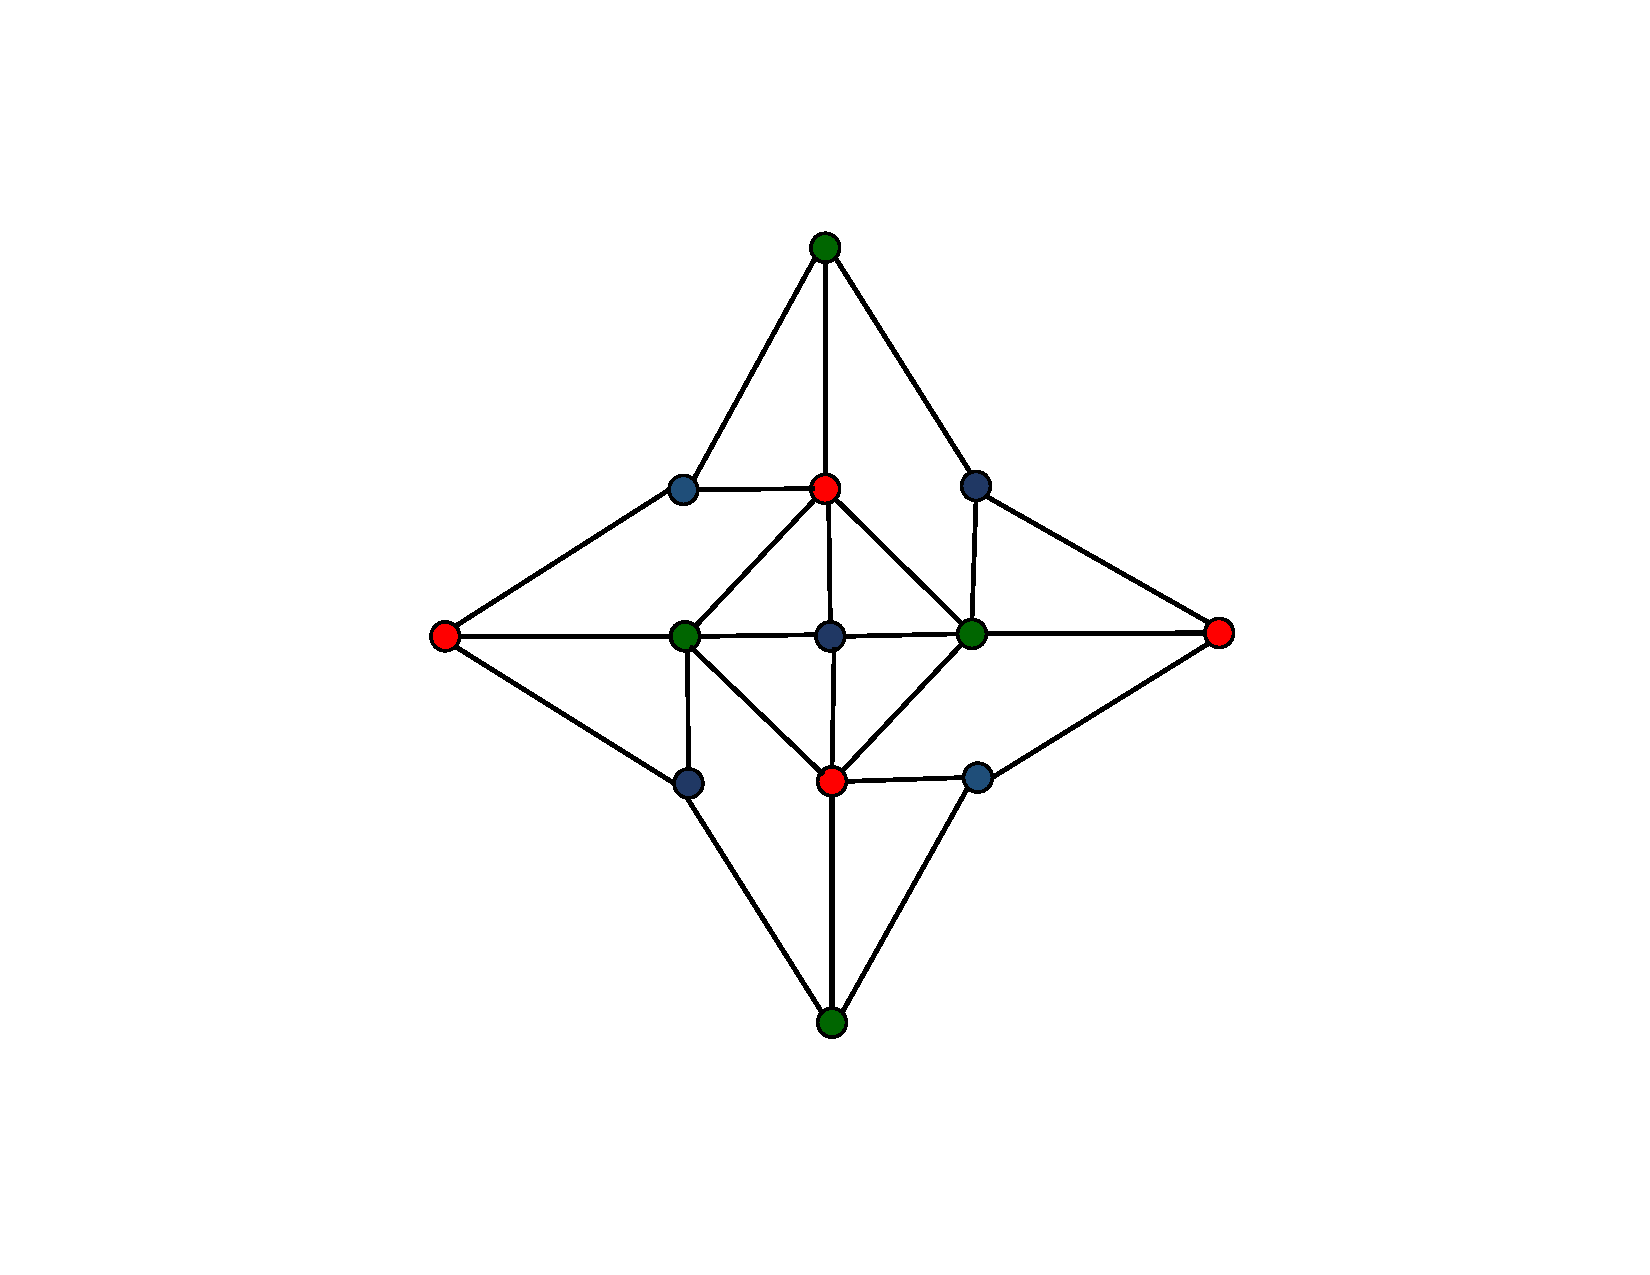
\includegraphics[width=4.0in]{3color-paterson-diff-color}
\caption{3-colorings for the gadget.}
\label{fig:3colorings}
\end{figure}
\end{solution}

\ppart Prove that the graph in Figure~\ref{fig:3color-gadget}
satisfies condition~\eqref{colors-cross}.

\hint The colorings for part~\eqref{verify3coloring} are almost
completely forced by the coloring of $u$ and $v$.

\begin{solution}
The 3-colorings for the same-color and different-color cases appear in
Figure~\ref{fig:3colorings}.

Once the three vertices of the topmost triangle of the gadget are
assigned different colors, and the leftmost vertex is assigned the
same color or different color as the topmost, the complete 3-colorings
are unique.  The reader should verify that this follows for the
same-color case because the colorings of successive vertices are
immediately forced by being adjacent to vertices already assigned to
different colors.

In the same-color case, the coloring is almost completely immediately
forced, except that there are two ways of the coloring the middle
three vertices that are not immediately forced.  One of these
middle-vertex colorings forces a successful coloring of the remaining
vertices as shown in Figure~\ref{fig:3colorings}.  The other possible
middle-vertex coloring eventually forces a pair of adjacent vertices
to have the same color, which rules it out.
\end{solution}

\eparts

\end{problem}

%%%%%%%%%%%%%%%%%%%%%%%%%%%%%%%%%%%%%%%%%%%%%%%%%%%%%%%%%%%%%%%%%%%%%
% Problem ends here
%%%%%%%%%%%%%%%%%%%%%%%%%%%%%%%%%%%%%%%%%%%%%%%%%%%%%%%%%%%%%%%%%%%%%

\endinput
